\documentclass[12pt, oneside]{book}

% Encoding and Font Packages
\usepackage[T1]{fontenc} % Enables more efficient encoding for characters
\usepackage[utf8]{inputenc} % Allows for direct input of Unicode characters
\usepackage{microtype} % Improves typography by fine-tuning text spacing

% Font Setup for Official Text
\usepackage{charter} % Primary font for readability
\usepackage{bm} 
\usepackage{mathpazo} 

% Monospaced Font for Code Listings
\usepackage[scaled=.95]{inconsolata}

% Color and Graphics
\usepackage{array}
\usepackage{xcolor} % For custom color definitions
\usepackage{graphicx} % To insert images, diagrams, etc.
\usepackage{caption} % Customization of figure captions
\usepackage{subcaption} % For sub-figures (helpful for detailed diagrams)
\usepackage{tikz} % For high-quality, custom diagrams and illustrations
\usetikzlibrary{positioning, shapes.geometric, arrows, calc} % Libraries for complex diagram creation

% Margins and Page Layout
\usepackage[a4paper, margin=1in]{geometry} % Adjust page margins
\usepackage{setspace} % For line spacing
\setstretch{1.3} % Sets a nice line spacing for the text (readable and clear)

% Headers and Footers
\usepackage{fancyhdr} % For fancy headers and footers
\pagestyle{fancy}
\fancyhf{}
\fancyhead[L]{\nouppercase{\leftmark}} % Left-aligned chapter heading
\fancyhead[R]{\thepage} % Right-aligned page number
\fancypagestyle{plain}{
	\fancyhf{}
	\fancyfoot[C]{\thepage} % Centered page number for "plain" pages
}

% Hyperlink and Navigation
\usepackage{hyperref} % For hyperlinks and navigation within the document
\hypersetup{
	colorlinks=true, % Enables colored links
	linkcolor=black, % Links are in black (good for printing)
	citecolor=blue, % Citation links are blue
	urlcolor=cyan, % URLs are cyan
	pdfauthor={Mahdi}, % Author metadata for PDF
	pdftitle={Arliz}, % Title metadata for PDF
	pdfsubject={Programming, Arrays, and Data Structures}, % Subject for PDF
	pdfkeywords={Arrays, Data Structures, Programming, History of Computing}, % Keywords for PDF
}

% Bibliography
\usepackage[backend=biber,style=apa]{biblatex} % APA-style citations
\addbibresource{references.bib} % Add the bibliography file

% Listings for Code
\usepackage{listings} % For code listings and syntax highlighting
\lstset{
	basicstyle=\ttfamily\small, % Monospaced font for code
	frame=single, % Draws a box around the code block
	breaklines=true, % Automatically breaks lines in code
	numbers=left, % Line numbers on the left
	numberstyle=\tiny\color{gray}, % Style of line numbers
	keywordstyle=\color{myblue}\bfseries, % Keywords in blue and bold
	commentstyle=\color{olive}, % Comments in green
	stringstyle=\color{orange}, % Strings in orange
	backgroundcolor=\color{lightgray!20}, % Light background for code blocks
	captionpos=b, % Position the caption at the bottom
	escapeinside={(*@}{@*)}, % Allows for inline LaTeX inside code blocks
	morekeywords={array, structure, algorithm, complexity}, % Add relevant keywords for highlighting
}

% Table of Contents and Index
\usepackage{tocbibind} % Adds bibliography and index to the table of contents
\usepackage{imakeidx} % For index generation
\makeindex % Generates the index

% Title Customization
\usepackage{titlesec} % For customizing chapter and section styles
\titleformat{\chapter}[display]
{\normalfont\huge\bfseries}{\chaptername\ \thechapter}{20pt}{\Huge}
\titleformat{\section}{\Large\bfseries}{\thesection}{1em}{}
\titleformat{\subsection}{\large\bfseries}{\thesubsection}{1em}{}

% Algorithms and Pseudocode
\usepackage{algorithm} % For displaying algorithms
\usepackage{algpseudocode} % For pseudocode formatting
% Special boxes and environments
\usepackage{tcolorbox}
\tcbuselibrary{most}

\newtcolorbox{notebox}[1][]{
	colback=blue!5!white,
	colframe=blue!75!black,
	title=Note,
	#1
}

\newtcolorbox{tipbox}[1][]{
	colback=green!5!white,
	colframe=green!75!black,
	title=Tip,
	#1
}

\newtcolorbox{warningbox}[1][]{
	colback=red!5!white,
	colframe=red!75!black,
	title=Important,
	#1
}
% Multicolumn for Glossary or Index
\usepackage{multicol} % For multicolumn layouts (useful for glossary)

% Custom Colors
\definecolor{myblue}{RGB}{0, 102, 204} % Define a custom blue color for code and links
\definecolor{lightgray}{RGB}{240, 240, 240} % Light gray for code backgrounds

% Title and author
% \title{{\Huge\textbf{Arliz}}\\[0.5em]
% {\LARGE A Journey Through Arrays and Computer Fundamentals}\\[1em]
%	{\large From Bits to Data Structures}}
% \author{{\LARGE Mahdi}} % Author name (Large font)
% \date{{\large \today}} % Date of the document
\usepackage{pdfpages}
\begin{document}
	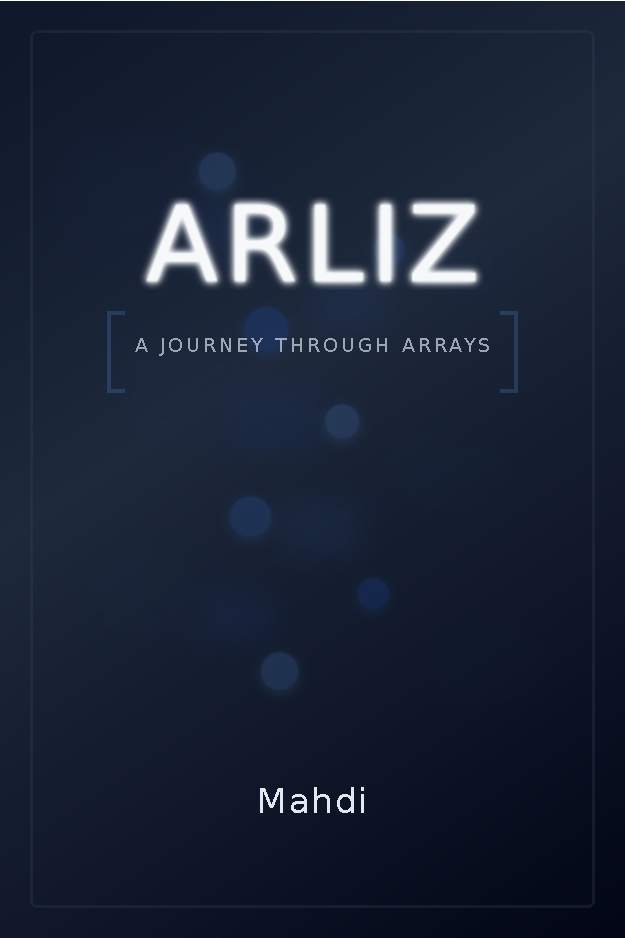
\includepdf[pages=-, pagecommand={}, width=\paperwidth, height=\paperheight]{logo.pdf}
	\frontmatter
	% Title Page (Front Matter)

\begin{titlepage}
	\begin{center}
		\vspace*{2cm}
		
		{\Huge\bfseries In Praise of Arliz}\\[2em]
		
		{\Large\scshape Mahdi}\\[0.5em]
		
		\begin{minipage}{1\textwidth}
			\centering
			This book evolves. Every insight gained—whether a circuit, a structure,\\
				or a simple idea—is absorbed and integrated. 
		\end{minipage}
		
		\vfill
		
	{\large \textsc{First Edition}}\\[0.5em]
	{\large \today}
	
	\vspace*{1cm}
	{\small
		\textcopyright\ 2025 Mahdi “Genix”  
		\par
		Released under the MIT License  
	}
	\end{center}
\end{titlepage}

%----------------------------------------------
% Dedication
%----------------------------------------------
\cleardoublepage
\thispagestyle{empty}
\vspace*{6cm}
\begin{center}
	\emph{
		To those who build from first principles.\\
		To the silent thinkers who design before they speak.\\
		To the ones who see in systems—\\
		not just machines, but metaphors.\\
		This is for you.}
\end{center}

	\chapter*{Preface}
	\thispagestyle{empty}
	\addcontentsline{toc}{chapter}{Preface}
	
	Every book has its own story, and this book is no exception. If I were to summarize the process of creating this book in one word, that word would be “improvised.” Yet the truth is that Arliz is the result of pure, persistent curiosity that has grown in my mind for years. What you are reading now could be called a technical book, a collection of personal notes, or even a journal of unanswered questions and curiosities. But I—officially—call it a \emph{book}, because it is written not only for others but for myself, as a record of my learning journey and an effort to understand more precisely the concepts that once seemed obscure and, at times, frustrating.\\
	The story of Arliz began with a simple feeling: \textbf{curiosity}.  
	Curiosity about what an array truly is. Perhaps for many this question seems trivial, but for me this word—encountered again and again in algorithm and data structure discussions—always raised a persistent question.\\
	Every time I saw terms like \texttt{array}, \texttt{stack}, \texttt{queue}, \texttt{linked list}, \texttt{hash table}, or \texttt{heap}, I not only felt confused but sensed that something fundamental was missing. It was as if a key piece of the puzzle had been left out. The first brief, straightforward explanations I found in various sources never sufficed; they assumed you already knew exactly what an array is and why you should use it. But I was looking for the \emph{roots}. I wanted to understand from zero what an array means, how it was born, and what hidden capacities it holds.\\
	That realization led me to decide:  
	\emph{If I truly want to understand, I must start from zero.}\\	
	There is no deeper story behind the name “Arliz.” There is no hidden philosophy or special inspiration—just a random choice. I simply declared:  
	\emph{This book is called Arliz.}  
	You may pronounce it "Ar-liz," "Array-Liz," or any way you like. I personally say "ar-liz." That is all—simple and arbitrary.\\	
	But Arliz is not merely a technical book on data structures. In fact, \textbf{Arliz grows alongside me}. \\
	Whenever I learn something I deem worth writing, I add it to this book. Whenever I feel a section could be explained better or more precisely, I revise it. Whenever a new idea strikes me—an algorithm, an exercise, or even a simple diagram to clarify a structure—I incorporate it into Arliz.\\
	This means Arliz is a living project. As long as I keep learning, Arliz will remain alive.\\	
	The structure of this book has evolved around a simple belief: true understanding begins with context. That’s why Arliz doesn’t start with code or syntax, but with the origins of computation itself. We begin with the earliest tools and ideas—counting stones, the abacus, mechanical gears, and early notions of logic—long before transistors or binary digits came into play. From there, we follow the evolution of computing: from ancient methods of calculation to vacuum tubes and silicon chips, from Babbage’s Analytical Engine to the modern microprocessor. Along this journey, we discover that concepts like arrays aren’t recent inventions—they are the culmination of centuries of thought about how to structure, store, and process information.\\
	In writing this book, I have always tried to follow three principles:
	
	\begin{itemize}
		\item \textbf{Simplicity of Expression:} I strive to present concepts in the simplest form possible, so they are accessible to beginners and not superficial or tedious for experienced readers.
		\item \textbf{Concept Visualization:} I use diagrams, figures, and visual examples to explain ideas that are hard to imagine, because I believe visual understanding has great staying power.
		\item \textbf{Clear Code and Pseudocode:} Nearly every topic is accompanied by code that can be easily translated into major languages like C\texttt{++}, Java, or C\#, aiming for both clarity and practicality.
	\end{itemize}
	
	An important note: many of the algorithms in Arliz are implemented by myself. I did not copy them from elsewhere, nor are they necessarily the most optimized versions. My goal has been to understand and build them from scratch rather than memorize ready-made solutions. Therefore, some may run slower than standard implementations—or sometimes even faster. For me, the process of understanding and constructing has been more important than simply reaching the fastest result.\\	
	Finally, let me tell you a bit about myself:  
	I am \textbf{Mehdi}. If you prefer, you can call me by my alias: \emph{Genix}. I am a student of Computer Engineering (at least at the time of writing this). I grew up with computers—from simple games to typing commands in the terminal—and I have always wondered what lies behind this screen of black and green text. There is not much you need to know about me, just that I am someone who works with computers, sometimes gives them commands, and sometimes learns from them.\\	
	I hope this book will be useful for understanding concepts, beginning your learning journey, or diving deeper into data structures. \\	
	Arliz is freely available. You can access the PDF, LaTeX source, and related code at:  
	\begin{center}
		\url{https://github.com/m-mdy-m/Arliz}
	\end{center}
	In each chapter, I have included exercises and projects to aid your understanding. Please do not move on until you have completed these exercises, because true learning happens only by solving problems.\\	
	I hope this book serves you well—whether for starting out, reviewing, or simply satisfying your curiosity. And if you learn something, find an error, or have a suggestion, please let me know. As I said:
	\emph{This book grows with me.}
	% Acknowledgments
	\chapter*{Acknowledgments}
	\thispagestyle{empty}
	\addcontentsline{toc}{chapter}{Acknowledgments}
	I would like to express my gratitude to everyone who supported me during the creation of this book. Special thanks to the open-source community for their invaluable resources and to all those who reviewed early drafts and provided feedback.
	
	%\maketitle
	\newpage
	\tableofcontents
	\renewcommand{\arraystretch}{1.5} % Adjust row height for better readability
	
	% Main Content
	\mainmatter

\part{The Birth of Computing: From Mechanical to Electronic}
\section*{Introduction}

Long before a single line of code was ever written—long before electricity, transistors, or even the concept of modern logic circuits—humans felt an innate drive to calculate, record, and model the world around them. Computing is not a recent invention. It is one of humanity’s oldest intellectual pursuits, rooted in necessity and evolved through creativity. Before we dive into complex abstractions like arrays or data structures, we must ask a deeper, almost philosophical question: \textbf{What does it mean to compute?}\\
This part of the book invites you on a journey—not just through the machinery and breakthroughs that brought us the modern computer, but through the evolution of human thought about numbers, representation, and control. Arrays, as we will later explore in depth, are not merely structures to store data. They are reflections of how we’ve ordered information for thousands of years. Their logic is built upon ancient insights—on sets, sequences, and patterns—and they embody the fundamental human need to represent, repeat, and manipulate structured information.\\
Our journey begins in ancient times, long before Christ, with devices like the abacus, first appearing over 2,500 years ago in Mesopotamia and later refined by Chinese, Roman, and Japanese cultures. The abacus was not just a calculator—it was an embodiment of the concepts of \textbf{state}, \textbf{position}, and \textbf{transformation}, principles that continue to underpin all modern computation. It allowed people to model quantities, track multiple values in parallel (an early echo of array indexing), and perform operations based on positional representation.\\
From these early tools, we progress into the classical mathematical age, where the Greeks formalized logic, and concepts like \textbf{sets} and \textbf{ordered lists} began to take philosophical shape. While not arrays in the modern sense, these ideas laid the intellectual groundwork for thinking about groups of data—grouped, related, or sequential—that could be acted upon as a whole. The set, in particular, became a foundational concept in mathematics and later in programming: an abstract container for elements that obey rules and enable operations. The leap from abstract sets to concrete arrays reflects one of the key transitions in computational history—from idea to implementation.\\
In the 17th century, visionaries like Blaise Pascal and Gottfried Wilhelm Leibniz attempted to automate arithmetic with mechanical devices. These weren’t just clever tools—they were the first signs of a dream to make thinking itself mechanical. Charles Babbage expanded this dream with his Analytical Engine in the 19th century, envisioning a machine that could be programmed and reprogrammed—a concept that wouldn’t become reality until a century later. Ada Lovelace, who worked with Babbage, went even further. She grasped that machines could go beyond numbers: they could process symbolic logic, follow instructions, and even imitate aspects of reasoning. She anticipated the algorithm as a mental construct, not just a set of steps.\\
As we move forward into the 20th century, the invention of electromechanical and electronic machines—using relays, vacuum tubes, and later transistors—marked a revolution. No longer limited by gears and levers, computers became faster, more reliable, and more abstract. The idea of a \textbf{stored program} emerged, allowing machines to modify their behavior dynamically. This wasn’t just a technical innovation—it was a conceptual transformation. Programs became data, and data became active. Arrays, now implemented in memory, could be changed, traversed, and manipulated at runtime—opening the door to software as we know it today.\\
Eventually, we arrive at logic gates, boolean algebra, and the transistor—the atomic units of modern computation. These are more than circuits; they are the physical embodiment of logical thought: conditions, branching, repetition. From gates we build circuits, from circuits microprocessors, and from those, machines that can simulate anything we can formalize.\\
Before concluding this part, we will look closely at how data is represented: binary numbers, encoding schemes, floating-point formats, and character representations. These are not just technical tools; they are perspectives. They define the limits of what a machine can know, express, and manipulate. And finally, we arrive at memory—where arrays live, grow, and function. Memory is not just storage; it is the canvas of computation. It is where change happens and where order emerges.\\
If you are excited to write code, build systems, and jump into implementation, you are free to skip ahead. But if you stay with us for this brief but essential historical and conceptual journey, you will see programming not just as control over a machine, but as part of a much older story: the story of how humans learned to structure thought, encode logic, and make abstract ideas come alive.\\
Let us begin—at the beginning. With sand, stone, wood, and brass. And with minds bold enough to imagine machines that think.

% ==========================================
% CHAPTER 1: PHILOSOPHICAL FOUNDATIONS
% ==========================================

\chapter{What Does It Mean to Compute?}

\section{The Human Urge to Measure and Represent}
\subsection{The Birth of Abstraction: From Reality to Symbol}
\subsection{Quantity, Quality, and the Need for Order}
\subsection{The Cognitive Origins of Structured Thinking}

\section{From Counting Stones to Conceptual Models}
\subsection{Tally Marks and Primitive State}
\subsubsection{The Concept of Discrete Representation}
\subsubsection{Position and Value: Early Insights}
\subsubsection{One-to-One Correspondence}

\subsection{Abstraction and the Birth of Mathematical Thought}
\subsubsection{From Concrete to Abstract Numbers}
\subsubsection{The Emergence of Zero and Infinity}
\subsubsection{Symbolic Manipulation vs. Physical Reality}

\section{Mathematical Roots of Arrays}
\subsection{Sets, Sequences, and Order}
\subsubsection{Euclid's Elements: Systematic Organization}
\subsubsection{The Concept of Mathematical Collections}
\subsubsection{Ordered vs. Unordered Structures}

\subsection{The Notion of Indexing and Mapping}
\subsubsection{Coordinate Systems in Ancient Mathematics}
\subsubsection{Positional Notation Systems}
\subsubsection{Functions and Mappings: Early Abstractions}

\subsection{From Euclid to Euler: Structure in Mathematical Systems}
\subsubsection{Systematic Proofs and Logical Sequences}
\subsubsection{Graph Theory and Relational Structures}
\subsubsection{The Bridge to Modern Data Organization}

% ==========================================
% CHAPTER 2: ANCIENT COMPUTING TOOLS
% ==========================================

\chapter{Ancient Tools of Structured Computation}

\section{The Abacus: Humanity's First Array-Like Structure}
\subsection{Mesopotamian Origins and Clay Tokens}
\subsubsection{Token Systems as Discrete Data Storage}
\subsubsection{Positional Value and Place Representation}
\subsubsection{The Transition from Tokens to Beads}

\subsection{Chinese Suanpan: Parallel Processing in Wood}
\subsubsection{Bi-quinary System Implementation}
\subsubsection{Multi-Column Operations and Carry Logic}
\subsubsection{The Art of Mental-Physical Coordination}

\subsection{Roman and Japanese Variants}
\subsubsection{Soroban: Precision and Efficiency}
\subsubsection{Cultural Adaptations and Regional Optimizations}
\subsubsection{Speed Computing Techniques}

\subsection{Philosophical Implications of the Abacus}
\subsubsection{State, Transformation, and Memory}
\subsubsection{Parallel Computation in Ancient Times}
\subsubsection{The Abacus as a Programming Interface}

\section{Ancient Number Tables: Proto-Arrays in Practice}
\subsection{Babylonian Mathematical Tablets}
\subsubsection{Multiplication Tables in Cuneiform}
\subsubsection{Square and Cube Root Tables}
\subsubsection{Astronomical Computation Tables}
\subsubsection{Two-Dimensional Data Organization}

\subsection{Egyptian Mathematical Papyri}
\subsubsection{Rhind Papyrus: Systematic Problem Solutions}
\subsubsection{Unit Fraction Tables and Decomposition}
\subsubsection{Geometric Progression Tables}
\subsubsection{Tabular Methods for Complex Calculations}

\section{Chinese Rod Numerals and Matrix Operations}
\subsection{The Rod Numeral System}
\subsubsection{Physical Representation of Abstract Numbers}
\subsubsection{Spatial Arrangement and Value}
\subsubsection{Early Binary-Like Concepts}

\subsection{Ancient Matrix Calculations}
\subsubsection{Simultaneous Linear Equations}
\subsubsection{The Nine Chapters on Mathematical Art}
\subsubsection{Gaussian Elimination in Ancient China}
\subsubsection{Matrix as a Computational Tool}

\subsection{Multiplication Matrices and Lookup Tables}
\subsubsection{Pre-computed Result Storage}
\subsubsection{Cross-Reference Systems}
\subsubsection{Error Checking and Verification Methods}

% ==========================================
% CHAPTER 3: MEDIEVAL AND RENAISSANCE
% ==========================================

\chapter{Medieval and Renaissance: Systematization of Knowledge}

\section{Islamic Golden Age Contributions}
\subsection{Al-Khwarizmi and Algorithmic thinking}
\subsubsection{The Word "Algorithm" and Its Origins}
\subsubsection{Systematic Problem-Solving Procedures}
\subsubsection{Algebra as Structured Manipulation}

\subsection{Mathematical Tables and Astronomical Calculations}
\subsubsection{Zij Tables: Astronomical Arrays}
\subsubsection{Trigonometric Function Tables}
\subsubsection{Precision and Interpolation Techniques}

\section{Renaissance Calculating Tools}
\subsection{Calculating Rods and Napier's Bones}
\subsubsection{John Napier's Logarithmic Innovation}
\subsubsection{Physical Implementation of Multiplication}
\subsubsection{Modular Arithmetic Tools}

\subsection{Mathematical Tables Revolution}
\subsubsection{Printed Logarithm Tables}
\subsubsection{Trigonometric Function Collections}
\subsubsection{Navigation and Scientific Computation}
\subsubsection{Error Propagation and Accuracy}

\section{The Emergence of Systematic Notation}
\subsection{Symbolic Algebra Development}
\subsubsection{François Viète and Symbolic Mathematics}
\subsubsection{The Power of Abstract Representation}
\subsubsection{From Numbers to Variables}

\subsection{Coordinate Systems and Cartesian Innovation}
\subsubsection{René Descartes and Analytical Geometry}
\subsubsection{Two-Dimensional Data Representation}
\subsubsection{Functions as Mappings}

% ==========================================
% CHAPTER 4: MECHANICAL COMPUTATION
% ==========================================

\chapter{Mechanical Computation: The Dream of Automated Thinking}

\section{Early Mechanical Calculators}
\subsection{Blaise Pascal's Pascaline}
\subsubsection{Mechanical Carry Implementation}
\subsubsection{Decimal Wheel Systems}
\subsubsection{The Challenge of Mechanical Precision}

\subsection{Leibniz's Stepped Reckoner}
\subsubsection{Four-Function Arithmetic Machine}
\subsubsection{The Leibniz Wheel Innovation}
\subsubsection{Mechanical Logic and Binary Concepts}

\section{Charles Babbage's Visionary Machines}
\subsection{The Difference Engine}
\subsubsection{Polynomial Calculation Automation}
\subsubsection{Method of Finite Differences}
\subsubsection{Precision Manufacturing Challenges}

\subsection{The Analytical Engine: First Programmable Computer}
\subsubsection{Separation of Processing and Memory}
\subsubsection{The Mill and the Store}
\subsubsection{Punched Card Programming}
\subsubsection{Conditional Branching and Loops}

\section{Ada Lovelace: The First Programmer}
\subsection{Understanding the Analytical Engine}
\subsubsection{Beyond Pure Calculation}
\subsubsection{Symbolic Processing Possibilities}
\subsubsection{The Concept of a Stored Program}

\subsection{Lovelace's Algorithm}
\subsubsection{Bernoulli Numbers Calculation}
\subsubsection{First Computer Program in History}
\subsubsection{Loop Structures and Iteration}

% ==========================================
% CHAPTER 5: ELECTROMECHANICAL ERA
% ==========================================

\chapter{The Electromechanical Revolution}

\section{From Mechanical to Electrical}
\subsection{Telegraph and Early Electrical Logic}
\subsubsection{Boolean Algebra in Physical Form}
\subsubsection{Relay-Based Switching Systems}
\subsubsection{Binary State Representation}

\subsection{Hollerith's Tabulating Machine}
\subsubsection{1890 US Census Automation}
\subsubsection{Punched Card Data Processing}
\subsubsection{Statistical Analysis Machines}

\section{Early 20th Century Computing Machines}
\subsection{Konrad Zuse's Z-Series}
\subsubsection{Z1: Mechanical Binary Computer}
\subsubsection{Z3: First Working Programmable Computer}
\subsubsection{Binary Floating-Point Arithmetic}
\subsubsection{Program Storage and Control}

\subsection{Harvard Mark I and IBM's Contribution}
\subsubsection{Electromechanical Programming}
\subsubsection{Grace Hopper and Early Programming}
\subsubsection{Large-Scale Scientific Computation}

% ==========================================
% CHAPTER 6: ELECTRONIC COMPUTING BIRTH
% ==========================================

\chapter{The Birth of Electronic Computing}

\section{The Vacuum Tube Revolution}
\subsection{From Mechanical to Electronic Switching}
\subsubsection{Thermionic Valve Principles}
\subsubsection{Digital Logic Implementation}
\subsubsection{Speed and Reliability Improvements}

\subsection{ENIAC: Electronic Numerical Integrator and Computer}
\subsubsection{First General-Purpose Electronic Computer}
\subsubsection{Programming by Rewiring}
\subsubsection{Parallel Processing Concepts}
\subsubsection{The Programming Challenge}

\section{The Stored Program Concept}
\subsection{Von Neumann Architecture}
\subsubsection{Programs as Data}
\subsubsection{Single Memory Space}
\subsubsection{Sequential Instruction Execution}
\subsubsection{The Fetch-Decode-Execute Cycle}

\subsection{EDVAC and the Architecture Revolution}
\subsubsection{Binary Number System Adoption}
\subsubsection{Memory Hierarchy Concepts}
\subsubsection{Subroutines and Program Structure}

% ==========================================
% CHAPTER 7: DIGITAL LOGIC FOUNDATIONS
% ==========================================

\chapter{Digital Logic: The Foundation of Modern Arrays}

\section{Boolean Algebra and Logical Operations}
\subsection{George Boole's Mathematical Logic}
\subsubsection{True/False as Mathematical Objects}
\subsubsection{AND, OR, NOT Operations}
\subsubsection{Logical Equivalence and Simplification}

\subsection{Claude Shannon's Digital Circuit Theory}
\subsubsection{Electrical Circuits as Logical Systems}
\subsubsection{Switching Theory and Boolean Algebra}
\subsubsection{The Bridge Between Math and Hardware}

\section{Transistors: The Atomic Units of Computation}
\subsection{From Vacuum Tubes to Solid State}
\subsubsection{Bell Labs and the Transistor Invention}
\subsubsection{Semiconductor Physics Basics}
\subsubsection{Switching Speed and Power Efficiency}

\subsection{Logic Gates Implementation}
\subsubsection{NAND and NOR as Universal Gates}
\subsubsection{Gate Delay and Propagation}
\subsubsection{Combinational vs. Sequential Logic}

\section{Building Complex Circuits}
\subsection{Adders and Arithmetic Logic Units}
\subsubsection{Half Adder and Full Adder}
\subsubsection{Ripple Carry vs. Look-Ahead}
\subsubsection{Multi-bit Operations}

\subsection{Memory Cells and Storage Elements}
\subsubsection{Flip-Flops and Latches}
\subsubsection{Static vs. Dynamic Memory}
\subsubsection{Address Decoding Logic}

% ==========================================
% CHAPTER 8: NUMBER SYSTEMS AND REPRESENTATION
% ==========================================

\chapter{Number Systems and Data Representation}

\section{Historical Counting Systems}
\subsection{Unary and Tally Systems}
\subsubsection{One-to-One Correspondence}
\subsubsection{Physical Limitation and Scaling}
\subsubsection{The Need for Positional Systems}

\subsection{Positional Number Systems}
\subsubsection{Babylonian Base-60 System}
\subsubsection{Decimal System Development}
\subsubsection{Binary Concepts in Ancient Cultures}

\section{Binary: The Language of Digital Machines}
\subsection{Why Binary for Digital Systems?}
\subsubsection{Physical Implementation Advantages}
\subsubsection{Noise Immunity and Reliability}
\subsubsection{Boolean Logic Correspondence}

\subsection{Binary Arithmetic Operations}
\subsubsection{Addition and Subtraction}
\subsubsection{Multiplication and Division}
\subsubsection{Bitwise Operations}

\subsection{Signed Number Representation}
\subsubsection{Sign-Magnitude Method}
\subsubsection{One's Complement System}
\subsubsection{Two's Complement: The Modern Standard}
\subsubsection{Overflow and Underflow Handling}

\section{Floating-Point: Representing the Continuous}
\subsection{Fixed-Point Limitations}
\subsubsection{Precision vs. Range Trade-offs}
\subsubsection{Scaling Problems in Computation}

\subsection{IEEE 754 Standard}
\subsubsection{Sign, Exponent, Mantissa Format}
\subsubsection{Normalization and Hidden Bit}
\subsubsection{Special Values: Infinity and NaN}
\subsubsection{Precision Levels: Single, Double, Extended}

\section{Character Encoding Evolution}
\subsection{From Morse Code to ASCII}
\subsubsection{Telegraph Encoding Systems}
\subsubsection{ASCII: American Standard Code}
\subsubsection{Extended ASCII Limitations}

\subsection{Unicode: Universal Character Representation}
\subsubsection{Multi-byte Encoding Systems}
\subsubsection{UTF-8, UTF-16, UTF-32 Formats}
\subsubsection{Internationalization Challenges}

% ==========================================
% CHAPTER 9: MEMORY ARCHITECTURE
% ==========================================

\chapter{Memory: The Canvas Where Arrays Live}

\section{Historical Storage Evolution}
\subsection{Physical Storage Media Timeline}
\subsubsection{Punched Cards and Paper Tape}
\subsubsection{Magnetic Drum Memory}
\subsubsection{Ferrite Core Memory}
\subsubsection{Semiconductor Memory Revolution}

\subsection{Storage Hierarchy Development}
\subsubsection{Access Time vs. Capacity Trade-offs}
\subsubsection{Cost per Bit Evolution}
\subsubsection{Volatility and Persistence}

\section{Modern Memory Architecture}
\subsection{Register Files and Cache Systems}
\subsubsection{CPU Register Organization}
\subsubsection{Cache Levels and Hierarchy}
\subsubsection{Cache Coherency Protocols}
\subsubsection{Translation Lookaside Buffers}

\subsection{Main Memory Organization}
\subsubsection{DRAM Technology and Refresh}
\subsubsection{Memory Banks and Interleaving}
\subsubsection{Error Correction Codes}
\subsubsection{Memory Controllers and Arbitration}

\section{Address Space and Virtual Memory}
\subsection{Physical vs. Virtual Addressing}
\subsubsection{Address Translation Mechanisms}
\subsubsection{Memory Management Units}
\subsubsection{Page Tables and Translation}

\subsection{Memory Protection and Isolation}
\subsubsection{Process Address Spaces}
\subsubsection{Segmentation and Paging}
\subsubsection{Access Control and Permissions}
\subsubsection{Address Space Layout Randomization}

\section{Memory Layout in Program Execution}
\subsection{Program Memory Segments}
\subsubsection{Code Segment (Text): Instruction Storage}
\subsubsection{Data Segment: Initialized Global Variables}
\subsubsection{BSS Segment: Uninitialized Data}
\subsubsection{Stack: Local Variables and Function Calls}
\subsubsection{Heap: Dynamic Memory Allocation}

\subsection{Memory Allocation Strategies}
\subsubsection{Static Allocation: Compile-Time Decisions}
\subsubsection{Stack Allocation: LIFO and Automatic Management}
\subsubsection{Heap Allocation: Dynamic and Flexible}
\subsubsection{Memory Pools and Custom Allocators}
\subsubsection{Garbage Collection Principles}

\section{Array Storage and Memory Layout}
\subsection{Contiguous Memory Allocation}
\subsubsection{Sequential Storage Benefits}
\subsubsection{Cache Locality and Performance}
\subsubsection{Memory Alignment Considerations}

\subsection{Multi-Dimensional Array Storage}
\subsubsection{Row-Major vs. Column-Major Layout}
\subsubsection{Address Calculation Formulas}
\subsubsection{Memory Access Patterns}

\subsection{Array Bounds and Safety}
\subsubsection{Buffer Overflow Vulnerabilities}
\subsubsection{Bounds Checking Mechanisms}
\subsubsection{Memory Safety Techniques}
	
% ==========================================
% PART 2: ARRAYS - THEORY TO IMPLEMENTATION
% ==========================================
\part{Array Odyssey: From Mathematical Abstraction to Computer Implementation}

\section*{Introduction}

Having traversed the historical landscape of computation—from ancient counting stones to modern silicon-based processors—we now stand at the threshold of understanding arrays not merely as programming constructs, but as fundamental mathematical objects that bridge abstract thinking and concrete implementation. This part of our journey transforms from the philosophical and historical to the rigorously technical, yet maintains the same spirit of deep understanding that has guided us thus far.\\
Arrays are not arbitrary programming conveniences. They are the digital manifestation of humanity's most basic cognitive operation: the organization of related information into structured, accessible patterns. When we defined arrays historically through Babylonian multiplication tables or Chinese calculation matrices, we were observing the same fundamental concept that now underlies virtually every computation performed by modern computers.\\
In this part, we will construct a complete understanding of arrays from multiple perspectives: mathematical, theoretical, implementational, and algorithmic. We begin with the mathematical foundations—set theory, functions, and formal definitions—that provide the rigorous framework for understanding what an array actually \emph{is} in the most fundamental sense. From there, we explore how these mathematical abstractions translate into physical reality through memory systems, addressing schemes, and hardware optimization techniques.\\
The journey continues into the rich ecosystem of array variants and specialized structures that computer scientists have developed to solve specific classes of problems. Dynamic arrays that grow and shrink, associative arrays that provide key-value mappings, bit arrays that compress boolean information, and sparse arrays that efficiently represent mostly-empty data—each represents a different solution to the fundamental challenge of organizing and accessing structured information.\\
Finally, we dive deep into the algorithmic universe that arrays enable. The fundamental operations of searching and sorting, the elegant patterns of two-pointer techniques and sliding windows, and the powerful framework of dynamic programming all become natural and intuitive when understood through the lens of array manipulation.\\
This part assumes you have absorbed the historical and conceptual foundation from Part I. If you have not, you may find some concepts challenging to grasp deeply, though the technical content remains accessible. The goal is not merely to teach you how to use arrays in programming languages, but to understand them so thoroughly that you could, if necessary, design and implement them from scratch on any computing system.\\
Let us begin this transformation from history to implementation, from concept to code.

% ==========================================
% CHAPTER 10: MATHEMATICAL FOUNDATIONS
% ==========================================

\chapter{Mathematical Foundations of Arrays}

\section{Formal Mathematical Definition}
\subsection{Arrays as Mathematical Functions}
\subsubsection{Domain and Codomain of Array Functions}
\subsubsection{Index Sets and Value Sets}
\subsubsection{Finite vs. Infinite Array Concepts}
\subsubsection{Partial Functions and Undefined Elements}

\subsection{Set-Theoretic Foundations}
\subsubsection{Arrays as Cartesian Products}
\subsubsection{Ordered Pairs and N-tuples}
\subsubsection{Relation Between Sets and Array Elements}
\subsubsection{Power Sets and Array Dimensions}

\subsection{Algebraic Structure of Arrays}
\subsubsection{Array Spaces as Vector Spaces}
\subsubsection{Linear Operations on Arrays}
\subsubsection{Scalar Multiplication and Addition}
\subsubsection{Inner Products and Array Metrics}

\section{Abstract Data Type Theory}
\subsection{ADT vs. Concrete Implementation}
\subsubsection{Interface Specification Principles}
\subsubsection{Behavioral Contracts and Invariants}
\subsubsection{Pre-conditions and Post-conditions}
\subsubsection{Abstract State vs. Physical Representation}

\subsection{Array ADT Specification}
\subsubsection{Core Operations: Create, Access, Update, Size}
\subsubsection{Optional Operations: Insert, Delete, Search}
\subsubsection{Composite Operations: Copy, Compare, Transform}
\subsubsection{Error Conditions and Exception Handling}

\subsection{Refinement and Implementation Relations}
\subsubsection{Data Refinement Theory}
\subsubsection{Abstraction Functions}
\subsubsection{Representation Invariants}
\subsubsection{Correctness of Implementations}

\section{Computational Complexity Theory}
\subsection{Big O Notation and Asymptotic Analysis}
\subsubsection{Growth Functions and Complexity Classes}
\subsubsection{Best, Average, and Worst-Case Analysis}
\subsubsection{Amortized Analysis Techniques}
\subsubsection{Space vs. Time Complexity Trade-offs}

\subsection{Array Operation Complexity}
\subsubsection{Random Access: O(1) Time Complexity}
\subsubsection{Sequential Access Patterns}
\subsubsection{Insert and Delete Operations}
\subsubsection{Memory Complexity Considerations}

\subsection{Lower Bounds and Optimality}
\subsubsection{Information-Theoretic Lower Bounds}
\subsubsection{Comparison-Based Operation Limits}
\subsubsection{Space-Time Trade-off Theory}
\subsubsection{Optimal Algorithm Design}

\section{Type Theory and Arrays}
\subsection{Homogeneous vs. Heterogeneous Arrays}
\subsubsection{Type Safety and Array Elements}
\subsubsection{Parametric Polymorphism}
\subsubsection{Generic Array Types}
\subsubsection{Type Inference in Array Operations}

\subsection{Index Type Systems}
\subsubsection{Integer Index Domains}
\subsubsection{Bounded vs. Unbounded Indices}
\subsubsection{Multi-dimensional Index Types}
\subsubsection{Dependent Types and Array Bounds}

\subsection{Memory Safety and Type Systems}
\subsubsection{Bounds Checking at Type Level}
\subsubsection{Linear Types and Memory Management}
\subsubsection{Ownership and Borrowing Models}
\subsubsection{Compile-time vs. Runtime Safety}

% ==========================================
% CHAPTER 11: PHYSICAL IMPLEMENTATION
% ==========================================

\chapter{Physical Implementation of Arrays}

\section{Memory Layout and Organization}
\subsection{Contiguous Memory Allocation}
\subsubsection{Sequential Address Assignment}
\subsubsection{Base Address and Offset Calculation}
\subsubsection{Memory Alignment Requirements}
\subsubsection{Padding and Structure Alignment}

\subsection{Address Calculation Formulas}
\subsubsection{One-Dimensional Array Indexing}
\subsubsection{Multi-Dimensional Array Formulas}
\subsubsection{Row-Major vs. Column-Major Layouts}
\subsubsection{Strided Arrays and Custom Layouts}

\subsection{Memory Hierarchy and Cache Performance}
\subsubsection{Cache Line Size and Array Access}
\subsubsection{Spatial Locality Optimization}
\subsubsection{Cache-Friendly Algorithm Design}
\subsubsection{False Sharing and Multi-threading}

\section{Static vs. Dynamic Array Implementation}
\subsection{Static Array Characteristics}
\subsubsection{Compile-Time Size Determination}
\subsubsection{Stack vs. Data Segment Allocation}
\subsubsection{Zero-Cost Abstractions}
\subsubsection{Template/Generic Instantiation}

\subsection{Dynamic Array Architecture}
\subsubsection{Runtime Size Modification}
\subsubsection{Heap-Based Memory Management}
\subsubsection{Growth Strategies and Capacity Management}
\subsubsection{Shrinking Policies and Memory Reclamation}

\subsection{Hybrid Approaches}
\subsubsection{Small Array Optimization}
\subsubsection{Stack-Allocated Dynamic Arrays}
\subsubsection{Memory Pool Allocation}
\subsubsection{Arena-Based Management}

\section{Multi-Dimensional Array Implementation}
\subsection{Linearization Strategies}
\subsubsection{Row-Major Order (C-style)}
\subsubsection{Column-Major Order (Fortran-style)}
\subsubsection{Block-Major and Tiled Layouts}
\subsubsection{Morton Order (Z-order)}

\subsection{Jagged Array Implementation}
\subsubsection{Array of Arrays Structure}
\subsubsection{Pointer Indirection Overhead}
\subsubsection{Memory Fragmentation Issues}
\subsubsection{Cache Performance Implications}

\subsection{Sparse Array Techniques}
\subsubsection{Coordinate List (COO) Format}
\subsubsection{Compressed Sparse Row (CSR)}
\subsubsection{Dictionary of Keys (DOK)}
\subsubsection{Block Sparse Representations}

\section{Hardware-Specific Optimizations}
\subsection{SIMD and Vector Processing}
\subsubsection{Vectorized Array Operations}
\subsubsection{Data Parallelism Exploitation}
\subsubsection{Alignment for Vector Instructions}
\subsubsection{Auto-Vectorization Techniques}

\subsection{GPU and Parallel Array Processing}
\subsubsection{CUDA Memory Hierarchy}
\subsubsection{Coalesced Memory Access}
\subsubsection{Shared Memory Optimization}
\subsubsection{Occupancy and Bandwidth Optimization}

\subsection{Non-Von Neumann Architectures}
\subsubsection{Dataflow Array Processing}
\subsubsection{Near-Memory Computing}
\subsubsection{Processing-In-Memory (PIM)}
\subsubsection{Neuromorphic Array Structures}

% ==========================================
% CHAPTER 12: ARRAY VARIANTS AND SPECIALIZATIONS
% ==========================================

\chapter{Array Variants and Specialized Structures}

\section{Dynamic Arrays and Resizable Structures}
\subsection{Vector/ArrayList Implementation}
\subsubsection{Capacity vs. Size Management}
\subsubsection{Geometric Growth Strategies}
\subsubsection{Amortized Analysis of Push Operations}
\subsubsection{Memory Reallocation Policies}

\subsection{Deque (Double-Ended Queue) Arrays}
\subsubsection{Circular Buffer Implementation}
\subsubsection{Block-Based Deque Design}
\subsubsection{Gap Buffer Techniques}
\subsubsection{Bi-directional Growth Strategies}

\subsection{Dynamic Array Optimization}
\subsubsection{Small Buffer Optimization}
\subsubsection{Copy-on-Write Strategies}
\subsubsection{Memory Pool Integration}
\subsubsection{Concurrent Dynamic Arrays}

\section{Associative Arrays and Hash-Based Structures}
\subsection{Hash Table Foundations}
\subsubsection{Hash Function Design}
\subsubsection{Collision Resolution Strategies}
\subsubsection{Open Addressing vs. Chaining}
\subsubsection{Load Factor and Performance}

\subsection{Advanced Hash Table Techniques}
\subsubsection{Robin Hood Hashing}
\subsubsection{Cuckoo Hashing}
\subsubsection{Consistent Hashing}
\subsubsection{Bloom Filters and Probabilistic Structures}

\subsection{Ordered Associative Arrays}
\subsubsection{Tree-Based Maps (Red-Black, AVL)}
\subsubsection{B+ Tree Array Implementation}
\subsubsection{Skip List Structures}
\subsubsection{Trie-Based Arrays}

\section{Bit Arrays and Compact Representations}
\subsection{Bit Vector Implementation}
\subsubsection{Bit-Level Operations}
\subsubsection{Word-Size Optimization}
\subsubsection{Population Count and Bit Manipulation}
\subsubsection{Set Operations on Bit Arrays}

\subsection{Bitmap Index Structures}
\subsubsection{Compressed Bitmaps}
\subsubsection{Roaring Bitmaps}
\subsubsection{WAH (Word-Aligned Hybrid) Compression}
\subsubsection{Bitmap Query Processing}

\subsection{Succinct Data Structures}
\subsubsection{Rank and Select Operations}
\subsubsection{Wavelet Trees}
\subsubsection{Compressed Suffix Arrays}
\subsubsection{Information-Theoretic Optimality}

\section{Circular Arrays and Ring Buffers}
\subsection{Circular Buffer Design}
\subsubsection{Head and Tail Pointer Management}
\subsubsection{Full vs. Empty Buffer Detection}
\subsubsection{Lock-Free Circular Buffers}
\subsubsection{Producer-Consumer Patterns}

\subsection{Specialized Circular Structures}
\subsubsection{Circular Array for Sliding Window}
\subsubsection{Circular Buffer for Real-Time Systems}
\subsubsection{Ring Buffer in Network Processing}
\subsubsection{Audio/Video Streaming Buffers}

\section{Sparse Arrays and Compressed Structures}
\subsection{Sparse Matrix Representations}
\subsubsection{Coordinate (COO) Format}
\subsubsection{Compressed Sparse Column (CSC)}
\subsubsection{Block Compressed Sparse Row}
\subsubsection{Diagonal Storage Schemes}

\subsection{Adaptive Sparse Structures}
\subsubsection{Dynamic Sparsity Detection}
\subsubsection{Hybrid Dense-Sparse Representations}
\subsubsection{Compressed Sensing Applications}
\subsubsection{Sparse Array Arithmetic}

\subsection{Specialized Compression Techniques}
\subsubsection{Run-Length Encoding for Arrays}
\subsubsection{Delta Compression}
\subsubsection{Dictionary-Based Compression}
\subsubsection{Lossy Array Compression}

% ==========================================
% CHAPTER 13: ARRAY ALGORITHMS AND PATTERNS
% ==========================================

\chapter{Fundamental Array Algorithms and Patterns}

\section{Search Algorithms}
\subsection{Linear Search Variants}
\subsubsection{Sequential Search Implementation}
\subsubsection{Sentinel-Based Linear Search}
\subsubsection{Binary Search for Sorted Arrays}
\subsubsection{Interpolation Search}
\subsubsection{Exponential Search}

\subsection{Advanced Search Techniques}
\subsubsection{Two-Pointer Search Patterns}
\subsubsection{Sliding Window Search}
\subsubsection{Subarray Search Problems}
\subsubsection{Pattern Matching in Arrays}

\subsection{Search Optimization}
\subsubsection{Branch Prediction Optimization}
\subsubsection{Cache-Friendly Search Algorithms}
\subsubsection{Parallel Search Strategies}
\subsubsection{Search in Specialized Arrays}

\section{Sorting Algorithms}
\subsection{Comparison-Based Sorting}
\subsubsection{Bubble Sort and Variants}
\subsubsection{Selection Sort Optimization}
\subsubsection{Insertion Sort and Binary Insertion}
\subsubsection{Shell Sort and Gap Sequences}

\subsection{Divide and Conquer Sorting}
\subsubsection{Merge Sort Implementation}
\subsubsection{Quick Sort and Pivot Selection}
\subsubsection{Heap Sort and Array-Based Heaps}
\subsubsection{Intro Sort Hybrid Approach}

\subsection{Non-Comparison Sorting}
\subsubsection{Counting Sort for Integer Arrays}
\subsubsection{Radix Sort Implementation}
\subsubsection{Bucket Sort Strategies}
\subsubsection{External Sorting for Large Arrays}

\subsection{Specialized Sorting}
\subsubsection{Stable vs. Unstable Sorting}
\subsubsection{In-Place Sorting Algorithms}
\subsubsection{Parallel Sorting Algorithms}
\subsubsection{Adaptive Sorting Techniques}

\section{Array Traversal Patterns}
\subsection{Basic Traversal Strategies}
\subsubsection{Forward and Backward Iteration}
\subsubsection{Nested Loop Patterns}
\subsubsection{Iterator-Based Traversal}
\subsubsection{Functional Programming Approaches}

\subsection{Two-Pointer Techniques}
\subsubsection{Convergent Two Pointers}
\subsubsection{Fast and Slow Pointers}
\subsubsection{Opposite Direction Pointers}
\subsubsection{Multiple Pointer Coordination}

\subsection{Sliding Window Algorithms}
\subsubsection{Fixed-Size Window Patterns}
\subsubsection{Variable-Size Window Techniques}
\subsubsection{Maximum/Minimum Window Problems}
\subsubsection{Substring/Subarray Applications}

\section{Dynamic Programming with Arrays}
\subsection{One-Dimensional DP}
\subsubsection{Fibonacci and Linear Recurrences}
\subsubsection{Maximum Subarray Problems}
\subsubsection{House Robber and Skip Patterns}
\subsubsection{Climbing Stairs Variations}

\subsection{Two-Dimensional DP}
\subsubsection{Grid Path Problems}
\subsubsection{Longest Common Subsequence}
\subsubsection{Edit Distance Algorithms}
\subsubsection{Matrix Chain Multiplication}

\subsection{Advanced DP Techniques}
\subsubsection{Space Optimization in DP}
\subsubsection{Rolling Array Techniques}
\subsubsection{State Compression Methods}
\subsubsection{Memoization vs. Tabulation}

\section{Array-Based Problem Solving Strategies}
\subsection{Greedy Algorithms on Arrays}
\subsubsection{Activity Selection Problems}
\subsubsection{Fractional Knapsack}
\subsubsection{Meeting Room Scheduling}
\subsubsection{Gas Station Problems}

\subsection{Divide and Conquer on Arrays}
\subsubsection{Maximum Subarray Sum}
\subsubsection{Closest Pair of Points}
\subsubsection{Inversion Count Problems}
\subsubsection{Peak Finding Algorithms}

\subsection{Backtracking with Arrays}
\subsubsection{Permutation Generation}
\subsubsection{Subset Generation}
\subsubsection{N-Queens Problem}
\subsubsection{Sudoku Solving Strategies}

\subsection{Mathematical Array Problems}
\subsubsection{Number Theory Applications}
\subsubsection{Combinatorial Problems}
\subsubsection{Probability and Statistics}
\subsubsection{Signal Processing Algorithms}

% ==========================================
% CHAPTER 14: LANGUAGE-SPECIFIC IMPLEMENTATIONS
% ==========================================

\chapter{Arrays in Programming Languages}

\section{Low-Level Language Implementations}
\subsection{C Language Arrays}
\subsubsection{Static Array Declaration and Initialization}
\subsubsection{Pointer Arithmetic and Array Access}
\subsubsection{Multi-dimensional Array Syntax}
\subsubsection{Array Decay to Pointers}
\subsubsection{Variable Length Arrays (C99)}

\subsection{C++ Array Enhancements}
\subsubsection{std::array for Fixed-Size Arrays}
\subsubsection{std::vector Dynamic Implementation}
\subsubsection{Template-Based Generic Arrays}
\subsubsection{RAII and Automatic Memory Management}
\subsubsection{Iterator and Range-Based Loops}

\subsection{Rust Memory-Safe Arrays}
\subsubsection{Ownership and Borrowing for Arrays}
\subsubsection{Stack vs. Heap Array Allocation}
\subsubsection{Vec<T> Dynamic Array Implementation}
\subsubsection{Compile-Time Bounds Checking}
\subsubsection{Zero-Cost Abstractions}

\section{High-Level Language Arrays}
\subsection{Python List Implementation}
\subsubsection{Dynamic Array with Object References}
\subsubsection{List Comprehensions and Generators}
\subsubsection{NumPy Arrays for Numerical Computing}
\subsubsection{Memory Layout and Performance}

\subsection{Java Array System}
\subsubsection{Primitive vs. Object Arrays}
\subsubsection{ArrayList and Dynamic Resizing}
\subsubsection{Multi-dimensional Array Implementation}
\subsubsection{Generics and Type Erasure}
\subsubsection{Collections Framework Integration}

\subsection{JavaScript Array Flexibility}
\subsubsection{Dynamic Typing and Mixed Arrays}
\subsubsection{Sparse Array Representation}
\subsubsection{Array Methods and Functional Programming}
\subsubsection{Typed Arrays for Binary Data}

\section{Functional Language Arrays}
\subsection{Haskell Immutable Arrays}
\subsubsection{Persistent Data Structures}
\subsubsection{Lazy Evaluation with Arrays}
\subsubsection{Array Comprehensions}
\subsubsection{Parallel Array Processing}

\subsection{Lisp-Family Languages}
\subsubsection{List as Primary Sequence Type}
\subsubsection{Vector Implementation in Clojure}
\subsubsection{Persistent Vector Tries}
\subsubsection{Structural Sharing}

\section{Domain-Specific Array Languages}
\subsection{MATLAB Array-Centric Design}
\subsubsection{Matrix as Fundamental Type}
\subsubsection{Vectorized Operations}
\subsubsection{Broadcasting and Element-wise Operations}
\subsubsection{Sparse Matrix Support}

\subsection{R Statistical Arrays}
\subsubsection{Vector and Matrix Types}
\subsubsection{Factor Arrays for Categorical Data}
\subsubsection{Data Frame as Columnar Arrays}
\subsubsection{Array-Oriented Statistical Functions}

\subsection{GPU Programming Languages}
\subsubsection{CUDA Array Memory Management}
\subsubsection{OpenCL Buffer Objects}
\subsubsection{Shader Language Array Types}
\subsubsection{Compute Shader Array Processing}
	
	\part{The Array Odyssey}
	 \chapter{Historical Emergence of Arrays}
	 \section{Early Array Concepts in Mathematics}
	 \section{Arrays in Assembly Language}
	 \subsection{IBM 704 Index Registers}
	 \section{Array Adoption in High-Level Languages}
	 
	 \chapter{Array Anatomy}
	 \section{Formal Mathematical Definition}
	 \section{Machine Representation}
	 \subsection{Contiguous Memory Layout}
	 \subsection{Stride and Cache Considerations}
	 \section{Dimensionality Perspectives}
	 \subsection{Physical vs. Logical Dimensions}
	 
	 \chapter{Memory Layout Engineering}
	 \section{Static Allocation Strategies}
	 \subsection{BSS vs. DATA Segments}
	 \section{Dynamic Allocation Mechanics}
	 \subsection{Heap Management Strategies}
	 \section{Multidimensional Mapping}
	 \subsection{Row-Major vs. Column-Major}
	 \subsection{Blocked Memory Layouts}
	 
	 \chapter{Array Indexing Evolution}
	 \section{Address Calculation Mathematics}
	 \subsection{Generalized Dimensional Formula}
	 \section{Bounds Checking Implementations}
	 \subsection{Hardware vs. Software Approaches}
	 \section{Pointer/Array Duality in C}
	 
	 \part{Advanced Array Concepts}
	 \chapter{Low-Level Optimization Techniques}
	 \section{Cache-Aware Array Traversal}
	 \section{SIMD Vectorization Strategies}
	 \section{False Sharing Prevention}
	 
	 \chapter{Theoretical Foundations}
	 \section{Arrays in Automata Theory}
	 \section{Turing Machines with Array Tapes}
	 \section{Chomsky Hierarchy Relationships}
	 
	 \chapter{Specialized Array Architectures}
	 \section{Sparse Array Storage}
	 \subsection{Compressed Sparse Row Format}
	 \section{Jagged Array Implementations}
	 \section{Associative Array Designs}

	 \chapter{Computer Architecture Supplement}
	 \section{From Vacuum Tubes to VLSI}
	 \section{Pipeline Architectures Deep Dive}
	 
	 \chapter{Number System Reference}
	 \section{Positional Number Proofs}
	 \section{Endianness Conversion Algorithms}
	 
	\chapter{Introduction to Arrays}
	\section{Overview}
	\section{Why Use Arrays?}
	\section{History}
	\chapter{Basics of Array Operations}
	\section{Traversal Operation}
	\section{Insertion Operation}
	\section{Deletion Operation}
	\section{Search Operation}
	\section{Sorting Operation}
	\section{Access Operation}
	\chapter{Types and Representations of Arrays}
	\section{Chomsky}
	\section{Types}
	\section{Abstract Arrays}
	\chapter{Memory Layout and Storage}
	\section{Memory Layout of Arrays}
	\section{Memory Segmentation and Bounds Checking}
	\subsection{Memory Segmentation}
	\subsubsection{Hardware Implementation}
	\subsubsection{Segmentation without Paging}
	\subsubsection{Segmentation with Paging}
	\subsubsection{Historical Implementations}
	\subsubsection{x86 Architecture}
	\subsection{Index-Bounds Checking}
	\subsubsection{Range Checking}
	\subsubsection{Index Checking}
	\subsubsection{Hardware Bounds Checking}
	\subsubsection{Support in High-Level Programming Languages}
	\subsubsection{Buffer Overflow}
	\subsubsection{Integer Overflow}
	\chapter{Development of Array Indexing}
	\subsubsection{Address Calculation for Multi-dimensional Arrays}
	\subsubsection{One-Dimensional Array}
	\subsubsection{Two-Dimensional Array}
	\subsubsection{Three-Dimensional Array}
	\subsubsection{Generalizing to a k-Dimensional Array}
	\subsubsection{Examples}
	\chapter{Array Algorithms}
	\section{Sorting Algorithms}
	\section{Searching Algorithms}
	\section{Array Manipulation Algorithms}
	\section{Dynamic Programming and Arrays}
	\chapter{Practical and Advanced Topics}
	\section{Self-Modifying Code in Early Computers}
	\section{Common Array Algorithms}
	\section{Performance Considerations}
	\section{Practical Applications of Arrays}
	\section{Future Trends in Array Handling}
	\chapter{Implementing Arrays in Low-Level Languages}
	\chapter{Static Arrays}
	\section{Single-Dimensional Arrays}
	\subsection{Declaration and Initialization}
	\subsection{Accessing Elements}
	\subsection{Iterating Through an Array}
	\subsection{Common Operations}
	\subsubsection{Insertion}
	\subsubsection{Deletion}
	\subsubsection{Searching}
	\subsection{Memory Considerations}
	\section{Multi-Dimensional Arrays}
	\subsection{2D Arrays}
	\subsubsection{Declaration and Initialization}
	\subsubsection{Accessing Elements}
	\subsubsection{Iterating Through a 2D Array}
	\subsection{3D Arrays and Higher Dimensions}
	\subsubsection{Declaration and Initialization}
	\subsubsection{Accessing Elements}
	\subsubsection{Use Cases and Applications}
	\chapter{Dynamic Arrays}
	\section{Introduction to Dynamic Arrays}
	\subsection{Definition and Overview}
	\subsection{Comparison with Static Arrays}
	
	\section{Single-Dimensional Dynamic Arrays}
	\subsection{Using \texttt{malloc} and \texttt{calloc} in C}
	\subsection{Resizing Arrays with \texttt{realloc}}
	\subsection{Using \texttt{ArrayList} in Java}
	\subsection{Using \texttt{Vector} in C++}
	\subsection{Using \texttt{List} in Python}
	
	\section{Multi-Dimensional Dynamic Arrays}
	\subsection{2D Dynamic Arrays}
	\subsubsection{Creating and Resizing 2D Arrays}
	\subsection{3D and Higher Dimensions}
	\subsubsection{Memory Allocation Techniques}
	\subsubsection{Use Cases and Applications}
	
	\chapter{Advanced Topics in Arrays}
	
	\section{Array Algorithms}
	\subsection{Sorting Algorithms}
	\subsubsection{Bubble Sort}
	\subsubsection{Merge Sort}
	\subsection{Searching Algorithms}
	\subsubsection{Linear Search}
	\subsubsection{Binary Search}
	
	\section{Memory Management in Arrays}
	\subsection{Static vs. Dynamic Memory}
	\subsection{Optimizing Memory Usage}
	
	\section{Handling Large Data Sets}
	\subsection{Efficient Storage Techniques}
	\subsection{Using Arrays in Big Data Applications}
	
	\section{Parallel Processing with Arrays}
	\subsection{Introduction to Parallel Arrays}
	\subsection{Applications in GPU Programming}
	
	\section{Sparse Arrays}
	\subsection{Representation and Usage}
	\subsection{Applications in Data Compression}
	\section{Multidimensional Arrays}
	\section{Jagged Arrays}
	\section{Sparse Arrays}
	\section{Array of Structures vs. Structure of Arrays}
	\section{Array-Based Data Structures}
	
	\chapter{Arrays in Theoretical Computing Paradigms}
	
	\section{Introduction to Theoretical Computing Paradigms}
	\section{Arrays in Turing Machines}
	\section{Arrays in Cellular Automata}
	\section{Arrays in Cellular Automata}
	\section{Arrays in Quantum Computing}
	\section{Arrays in Neural Network Simulations}
	\section{Arrays in Automata Theory}
	\section{Arrays in Hypercomputation Models}
	\section{The Lambda Calculus Perspective on Arrays}
	\section{Arrays in Novel Computational Models}
	
	\chapter{Specialized Arrays and Applications}
	\section{Circular Buffers}
	\section{Circular Arrays}
	\subsection{Implementation and Use Cases}
	\subsection{Applications in Buffer Management}
	
	\section{Dynamic Buffering and Arrays}
	\subsection{Dynamic Circular Buffers}
	\subsection{Handling Streaming Data}
	
	\section{Jagged Arrays}
	\subsection{Definition and Usage}
	\subsection{Applications in Database Management}
	
	\section{Bit Arrays (Bitsets)}
	\subsection{Introduction and Representation}
	\subsection{Applications in Cryptography}
	\section{Circular Buffers}
	\section{Priority Queues}
	\section{Hash Tables}
	\section{Bloom Filters}
	\section{Bit Arrays and Bit Vectors}
	
	\chapter{Linked Lists}
	\section{Overview}
	\section{Singly Linked Lists}
	\section{Doubly Linked Lists}
	\section{Circular Linked Lists}
	\section{Comparison with Arrays}
	
	\chapter{Array-Based Algorithms}
	\section{Sorting Algorithms}
	\section{Searching Algorithms}
	\section{Array Manipulation Algorithms}
	\section{Dynamic Programming and Arrays}
	
	\chapter{Performance Analysis}
	\section{Time Complexity of Array Operations}
	\section{Space Complexity Considerations}
	\section{Cache Performance and Optimization}
	
	\chapter{Memory Management}
	\section{Memory Allocation Strategies}
	\section{Garbage Collection}
	\section{Manual Memory Management in Low-Level Languages}
	
	\chapter{Error Handling and Debugging}
	\section{Common Errors with Arrays}
	\section{Bounds Checking Techniques}
	\section{Debugging Tools and Strategies}
	
	\chapter{Optimization Techniques for Arrays}
	\section{Optimizing Array Traversal}
	\section{Minimizing Cache Misses}
	\section{Loop Unrolling}
	\section{Vectorization}
	\section{Memory Access Patterns}
	\section{Reducing Memory Fragmentation}
	
	\chapter{Concurrency and Parallelism}
	\section{Concurrent Array Access}
	\section{Parallel Array Processing}
	\section{Synchronization Techniques}
	
	\chapter{Applications in Modern Software Development}
	\section{Arrays in Graphics and Game Development}
	\section{Arrays in Scientific Computing}
	\section{Arrays in Data Analysis and Machine Learning}
	\section{Arrays in Embedded Systems}
	
	\chapter{Arrays in High-Performance Computing (HPC)}
	\section{Introduction to HPC Arrays}
	\section{Distributed Arrays}
	\section{Parallel Processing with Arrays}
	\section{Arrays in GPU Computing}
	\section{Multi-threaded Array Operations}
	\section{Handling Arrays in Cloud Computing}
	
	\chapter{Arrays in Functional Programming}
	\section{Immutable Arrays}
	\section{Persistent Arrays}
	\section{Arrays in Functional Languages (Haskell, Erlang, etc.)}
	\section{Functional Array Operations}
	
	\chapter{Arrays in Machine Learning and Data Science}
	\section{Numerical Arrays}
	\section{Handling Large Datasets with Arrays}
	\section{Arrays in Tensor Operations}
	\section{Arrays in Dataframes}
	\section{Optimization of Array-Based Algorithms in ML}
	
	\chapter{Advanced Memory Management in Arrays}
	\section{Memory Pools}
	\section{Dynamic Memory Allocation Strategies}
	
	\chapter{Data Structures Derived from Arrays}
	\section{Stacks}
	\section{Queues}
	\section{Heaps}
	\section{Hash Tables}
	\section{Trees Implemented Using Arrays}
	\section{Graphs Implemented Using Arrays}
	\section{Dynamic Arrays as Building Blocks}
	
	\chapter{Best Practices and Common Pitfalls in Array Usage}
	\section{Avoiding Out-of-Bounds Errors}
	\section{Efficient Initialization}
	\section{Choosing the Right Array Type}
	\section{Debugging and Testing Arrays}
	\section{Avoiding Memory Leaks}
	\section{Ensuring Portability Across Platforms}
	
	\chapter{Historical Perspectives and Evolution}
	\section{Custom Memory Allocators}\section{Early Implementations}
	\section{Array Storage on Disk}\section{Evolution of Array Data Structures}
	\section{Impact on Programming Languages and Paradigms}
	
	\chapter{Future Trends in Array Handling}
	\section{Emerging Data Structures}
	\section{Quantum Computing and Arrays}
	\section{Bioinformatics Applications}
	\section{Big Data and Arrays}
	\section{Arrays in Emerging Programming Paradigms}
	\chapter{Appendices}
	\section{Glossary of Terms}
	\section{Bibliography}
	\section{Index}
	
% References
\printbibliography[heading=bibintoc]

% Index
\printindex
\end{document}